\section{Introductions}
In a typical tumour xenograft experiment, the animals are randomised between the control and treatment lines.
Once human tumour samples are administrated on the animals on both groups, the responses are monitored over the follow-up period resulting in a set of individual trajectories within each treatment line.
If the tumour size exceeds the level where further continuation of the experiment is against animal welfare conventions, the animal is culled.
The experiment stops once the end of follow-up period is reached.
The resulting sample have a longitudinal form, where at each time point there is a set of the tumour measurements recorded for the alive animals in the sample over the follow-up period.
\Cref{raw_trajectories} shows a typical outcome of such experiment outcome represented with the tumour volume changes over time.

\begin{figure}
	\centering
	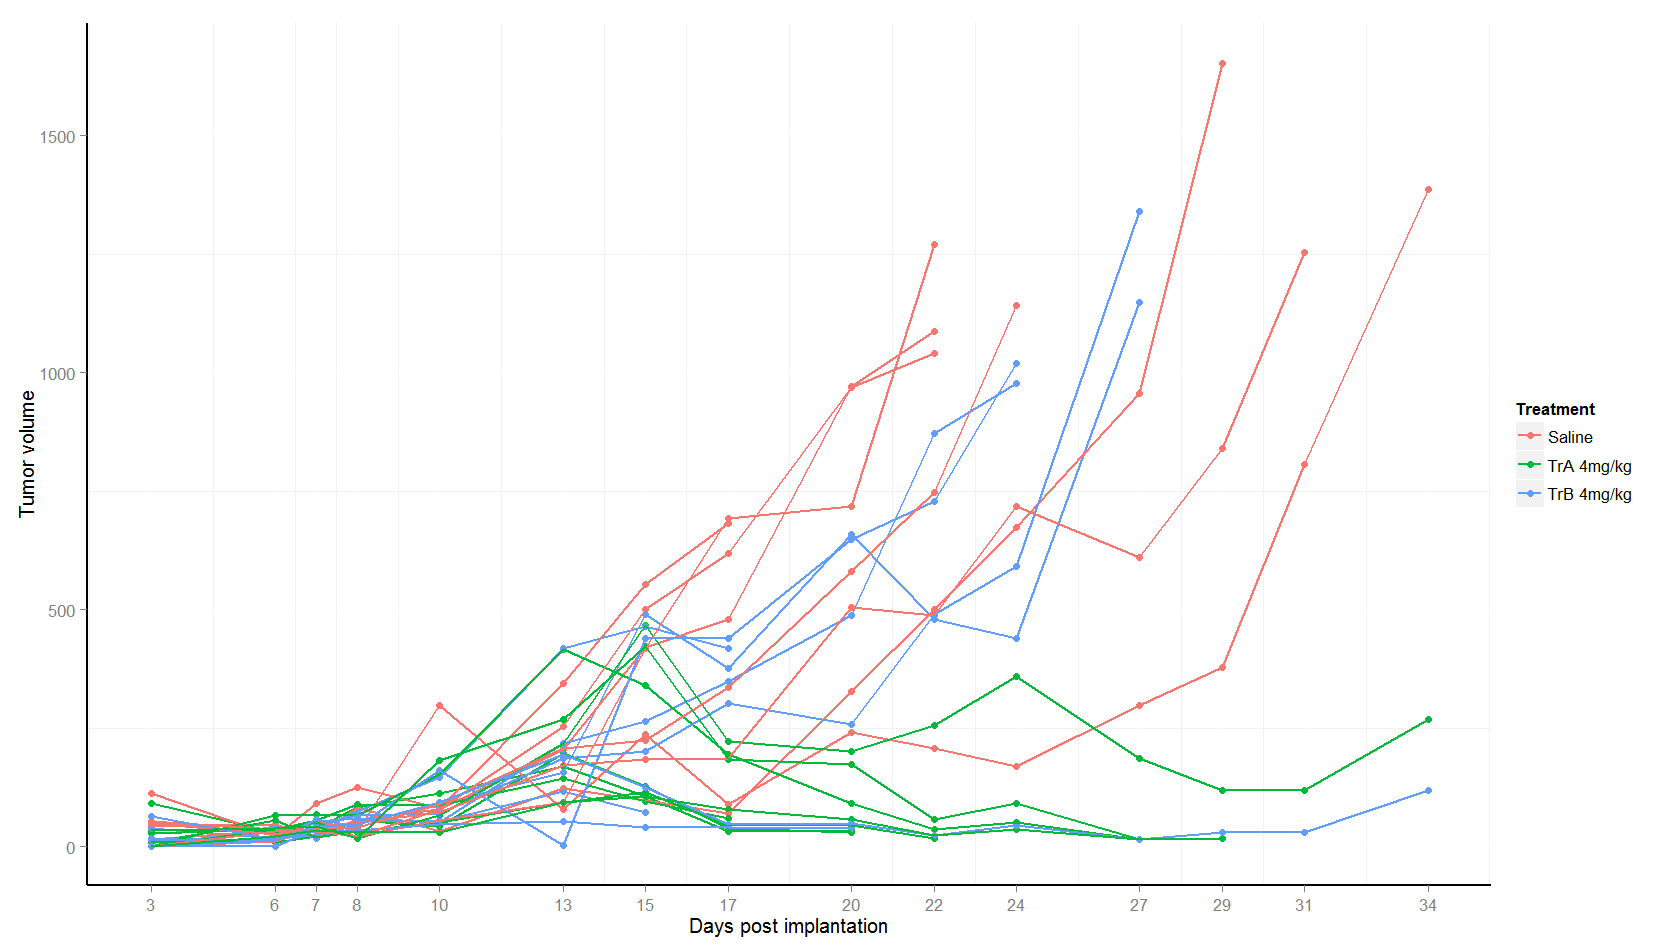
\includegraphics[width=\textwidth]{xenograph/figures/raw_trajectories.png}
	\caption{Empirical tumour volume (mm$^3$) trajectories from \emph{in-vivo} tumour xenograft experiment.}
	\label{raw_trajectories}
\end{figure}

The observed differences between the measurements in the control and treatment groups constitute the therapy effectiveness.
The therapies can differ in terms of the dose level or active agent type or both.
The interest might be also in a differences between therapy lines.
In majority of cases, the resulting tumour volume data frequently exhibit heterogeneous responses with numerous outliers and hardly linear growth patterns.
Therefore, statistical assessment of the therapy effectiveness becomes a challenging task.

\section{The data}
\subsection{Selection of empirical evidence}
The tumour volume readings as a response to therapies may be a subject for selection before the statistical analysis of treatment effects is carried out.
For the analysed sample the period between day 6 and day 27 was selected.
The beginning of the sample corresponds to the day the animals got randomised to the control (Saline) and Treatment lines.
The last day of the selected sample is the last time-point where at least two tumour volume readings are available for each animal.

\begin{figure}
	\centering
	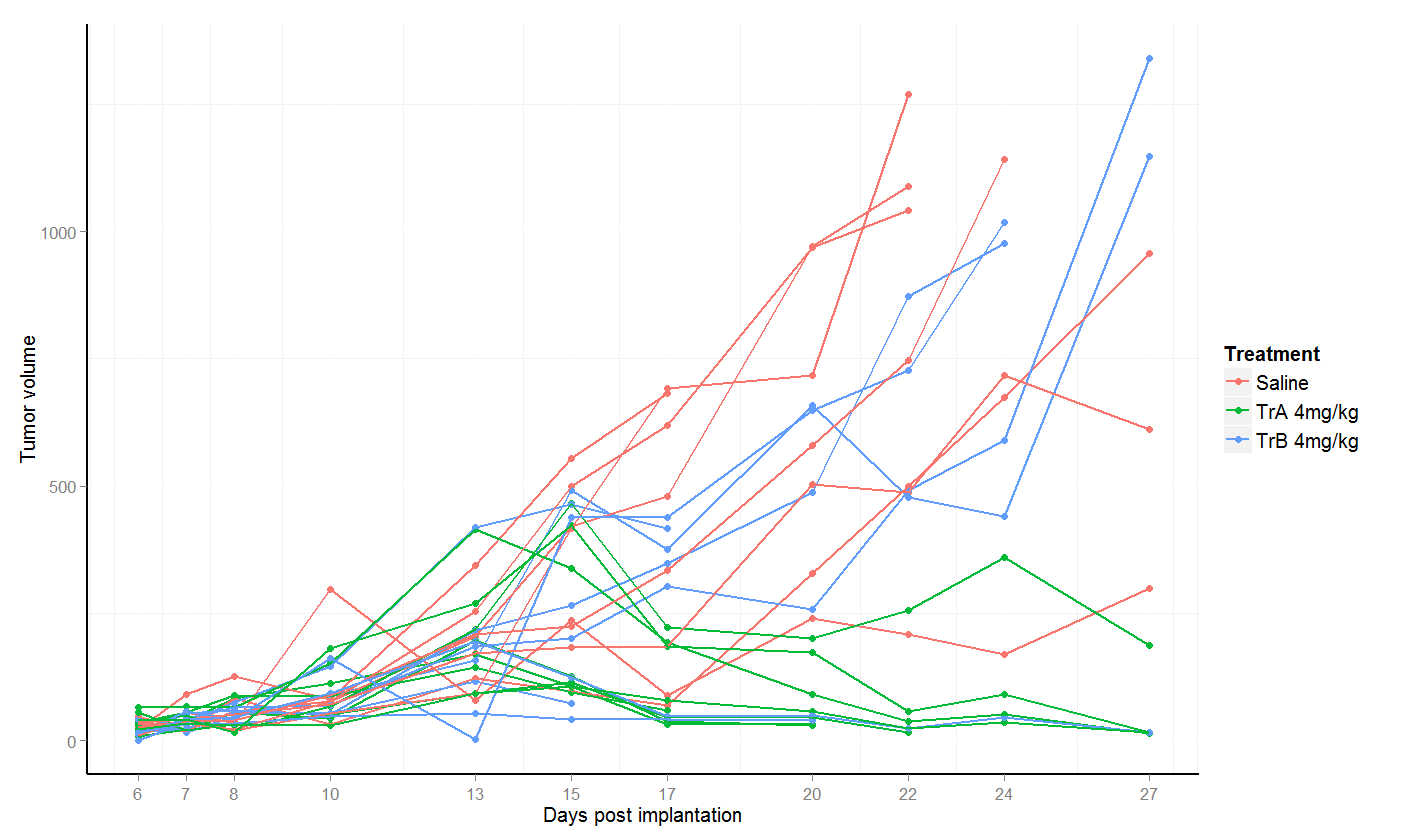
\includegraphics[width=\textwidth]{xenograph/figures/raw_trajectories_reduced.png}
	\caption{Empirical tumour volume (mm$^3$) trajectories from \emph{in-vivo} tumour xenograft experiment for selected time-points.}
	\label{raw_trajectories_reduced}
\end{figure}

\subsection{Exponential tumour growth}

Mathematical models of tumour growth are numerous and come in various levels of complexity.
Many of these models use a combination of partial and ordinary differential equations, these models have the ability to display multiple stages of tumour growth and can represent very complicated dynamics of both individual tumours and populations of tumours.
These models, while sophisticated, generally require a great deal of training data for adequate parameterisation and this can become inadequate when resources are limited to small data sets.

The Gompertz model \autocite{Norton1976} has been shown as an accurate model for tumour growth over time but an even simpler model would be one of basic exponential growth.
An exponential growth model can be considered to be a good approximation to Gompertz during the phase of tumour growth where the rate of growth is fastest (the second stage out of 3).
In practice this second stage of growth is the one of most experimental interest as during the early stages the tumours are hard to detect and in the later stages the tumour has developed too far and the subject would be culled.
In the next section we will discuss the benefits to data analysis when the data is approximately normally distributed (Gaussian in shape).
Tumour growth data tends to have a distribution with a long tail \cref{tumour_data} which gives us reason to believe that it follows an exponential growth pattern.

\begin{figure}
\centering
\begin{subfigure}{.49\textwidth}
	\centering
	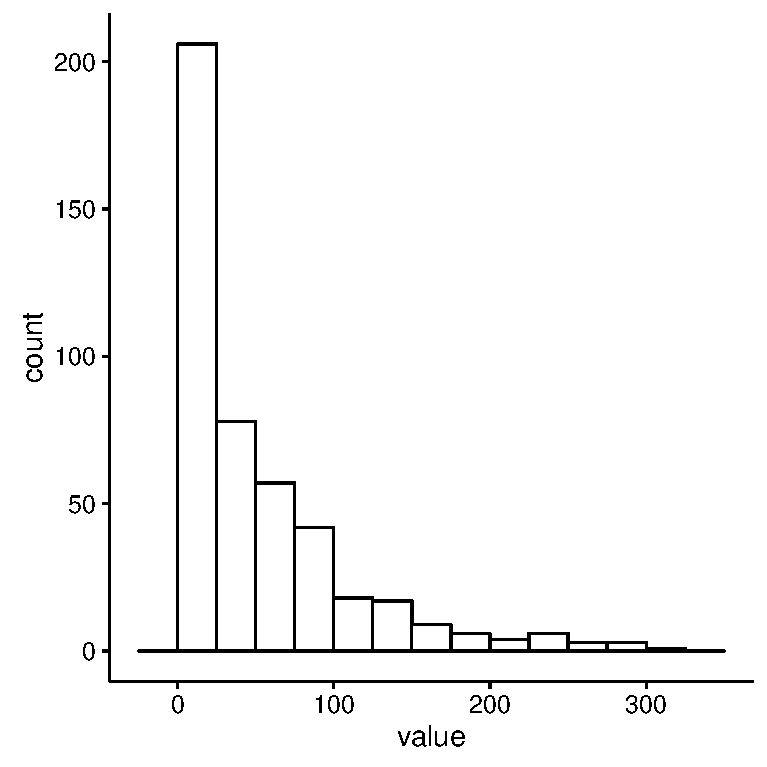
\includegraphics[width=\linewidth]{xenograph/normalisation/data_hist.pdf}
	\caption{Sample data on the original scale.}
	\label{tumour_data}
\end{subfigure}
\begin{subfigure}{.49\textwidth}
	\centering
	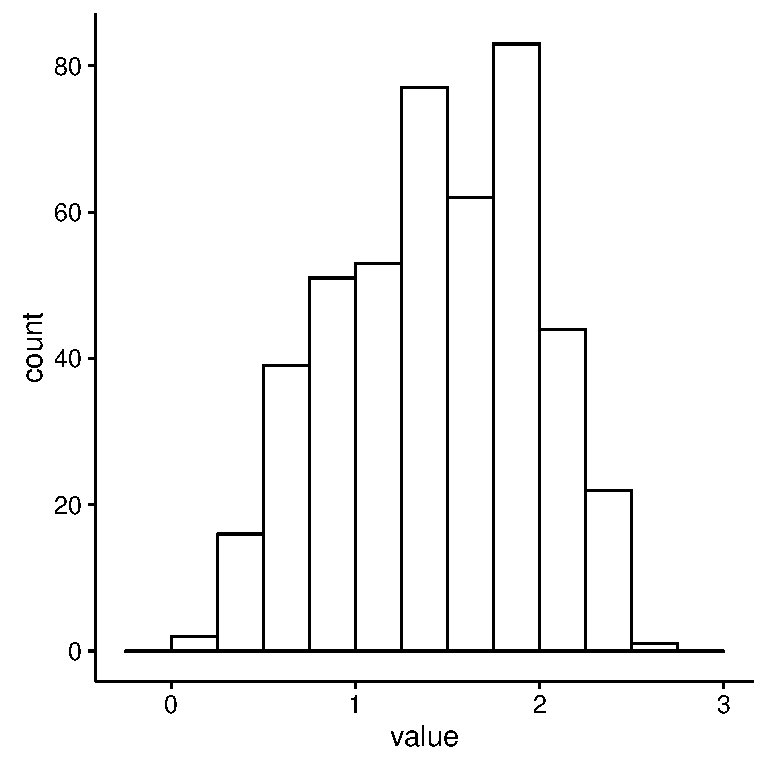
\includegraphics[width=\linewidth]{xenograph/normalisation/log_data_hist.pdf}
	\caption{The same data on the log$_{10}$ scale}
	\label{log_tumour_data}
\end{subfigure}
\caption{Showing that the log transform presents the synthetic data as more symmetrical and  $'$more gaussian$'$, this will make any statistical methods more powerful due to assumptions of normality}
\label{tumour_histograms}
\end{figure}

\subsection{Normalisation}
It is recommended that the tumour volume data get normalised before the visual and representative analysis is carried out \autocite{Heitjan:1993uw,Demidenko:2010gn}.
Tumour volume distribution is usually skewed and influenced by the outliers, in particular if sample is small, leading to imprecise outcomes and power reductions.
Making the distribution more Gaussian looking helps in reducing this bias and leads to a better power and more statistically significant treatment effects.
The most popular normalising technique is a log-transformation.
It is stabilising the tumour volume variance and given its monotonic property it does not affect the data content.
Therefore it is recommended but may require results to be back-transformed once interpreted.
\Cref{raw_trajectories_log_reduced_follow-up} presents the log$_{10}$-transformed original data (see \cref{raw_trajectories}) over the selected follow-up sub-period.
Given that the log function is not defined for zero volumes they needs to be imputed as zeros on a log-scale.
The follow-up period was reduced to the most relevant part.
It starts on day 6 when the animals get randomised among the treatment groups, and ends-up on day 27 where there are at least two alive animals per treatment line.
The log-transformed trajectories present an exponential growth pattern.


\begin{figure}
	\centering
	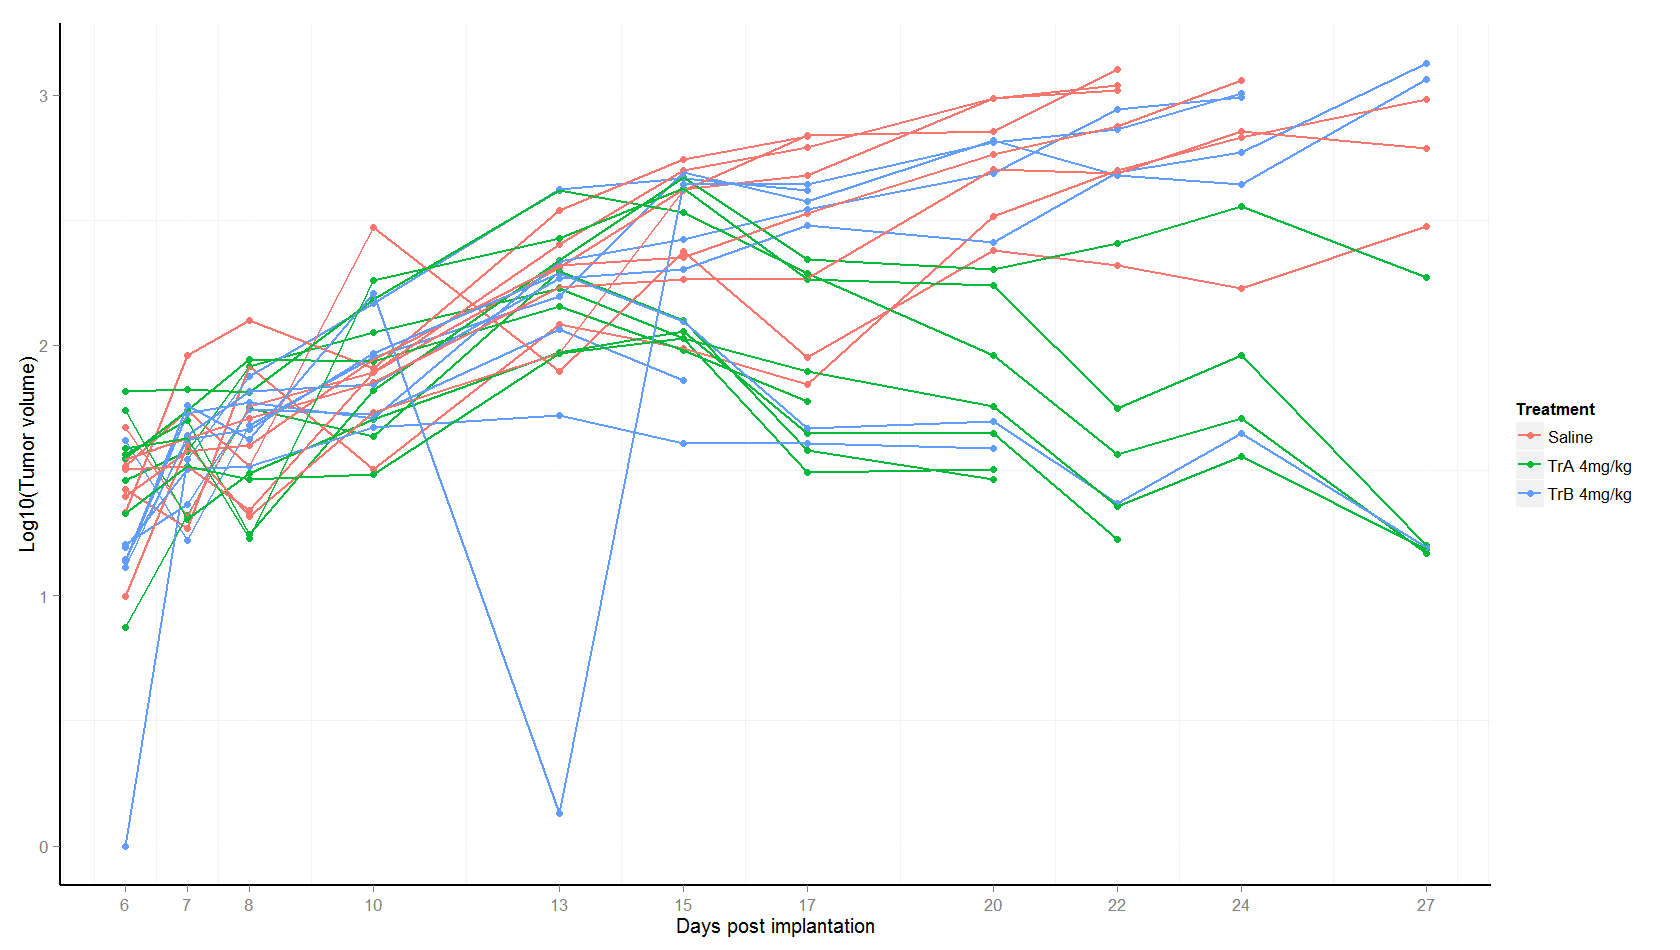
\includegraphics[width=\textwidth]{xenograph/figures/raw_trajectories_log_reduced_follow-up.png}
	\caption{Empirical tumour volume (mm$^3$) trajectories after log$_{10}$-transformation.}
	\label{raw_trajectories_log_reduced_follow-up}
\end{figure}

\subsection{Imputation}
The xenograft experiments do not provide complete longitudinal samples.
The prominent part stands for informed missing outcomes, resulting from the cases when tumours reach the levels where due to ethical reasons animal needs to be culled.
Reduced sample may be a problem for some statistical techniques, which require balanced samples.
The analysis might be carried out on reduced empirical evidence, which limits representativeness of the outcomes.
Alternatively, the informed missing data can be imputed to increase eligibility of available sample evidence for statistical testing.
However, it may lead to misleading or contradictory outcomes regarding treatment effect.
\Cref{error_bars_log_reduced_follow-up,error_bars_log_LOCF_reduced_follow-up} provide the mean and standard error bars for the raw tumour volume data and after the last-observation-carried-forward (LOCF) imputation applied, respectively.

\begin{figure}
	\centering
	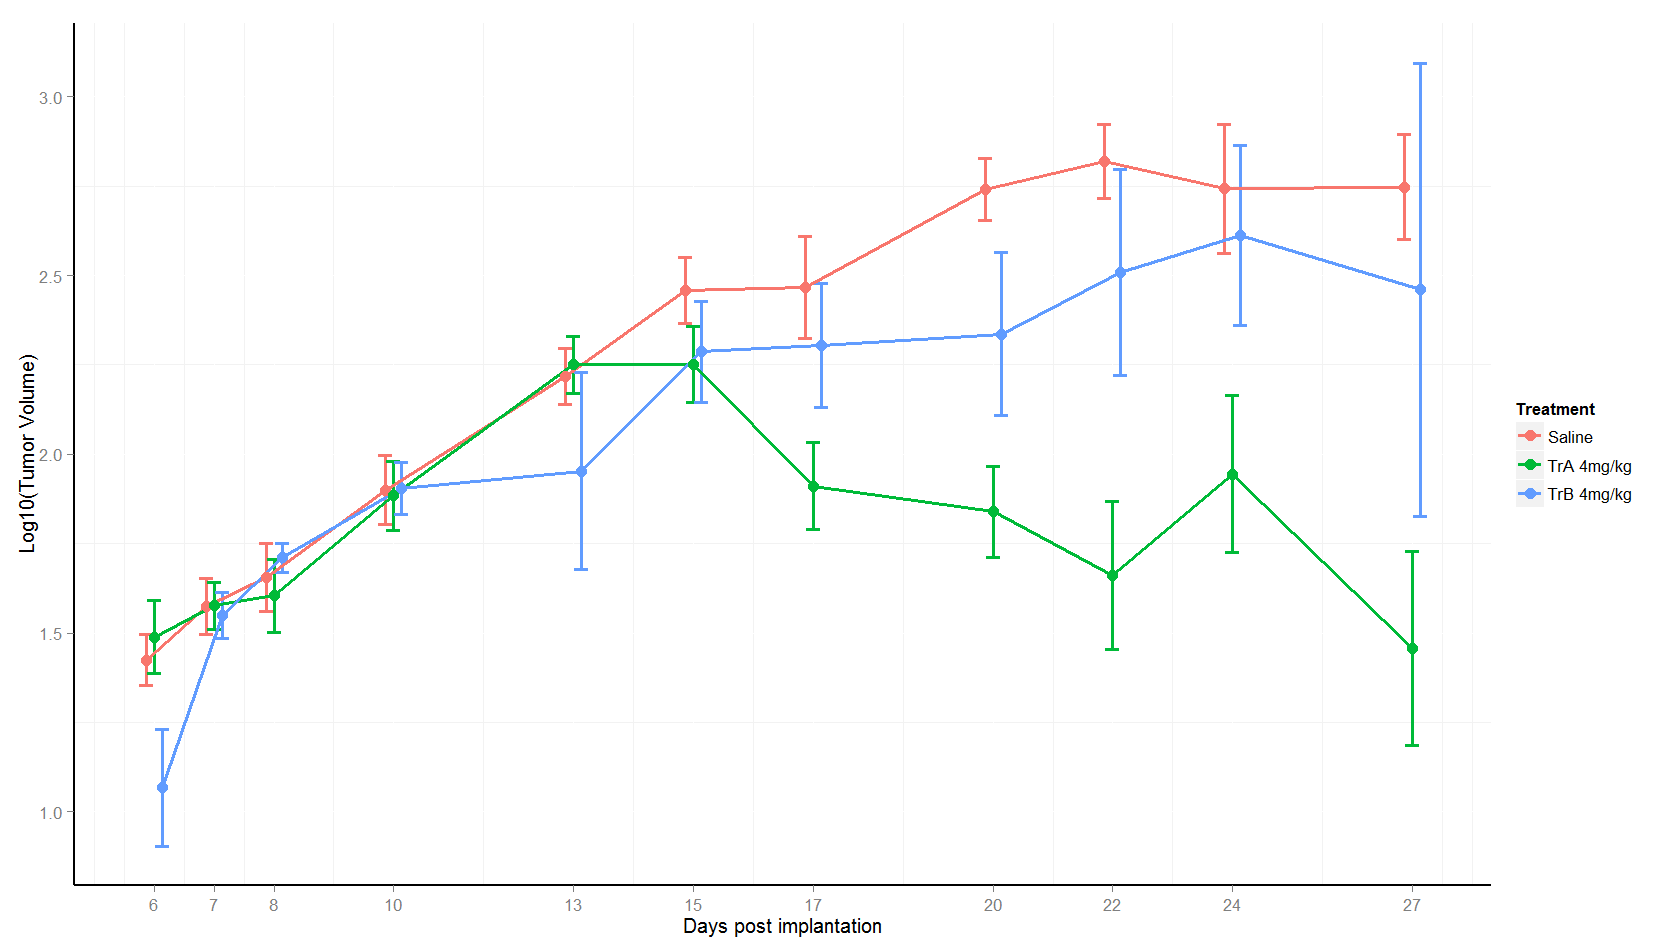
\includegraphics[width=\textwidth]{xenograph/figures/error_bars_log_reduced_follow-up.png}
	\caption{Mean log$_{10}$-transformed tumour volume (mm$^3$) and standard errors for particular treatment lines over the follow-up time-points.}
	\label{error_bars_log_reduced_follow-up}
\end{figure}

\begin{figure}
	\centering
	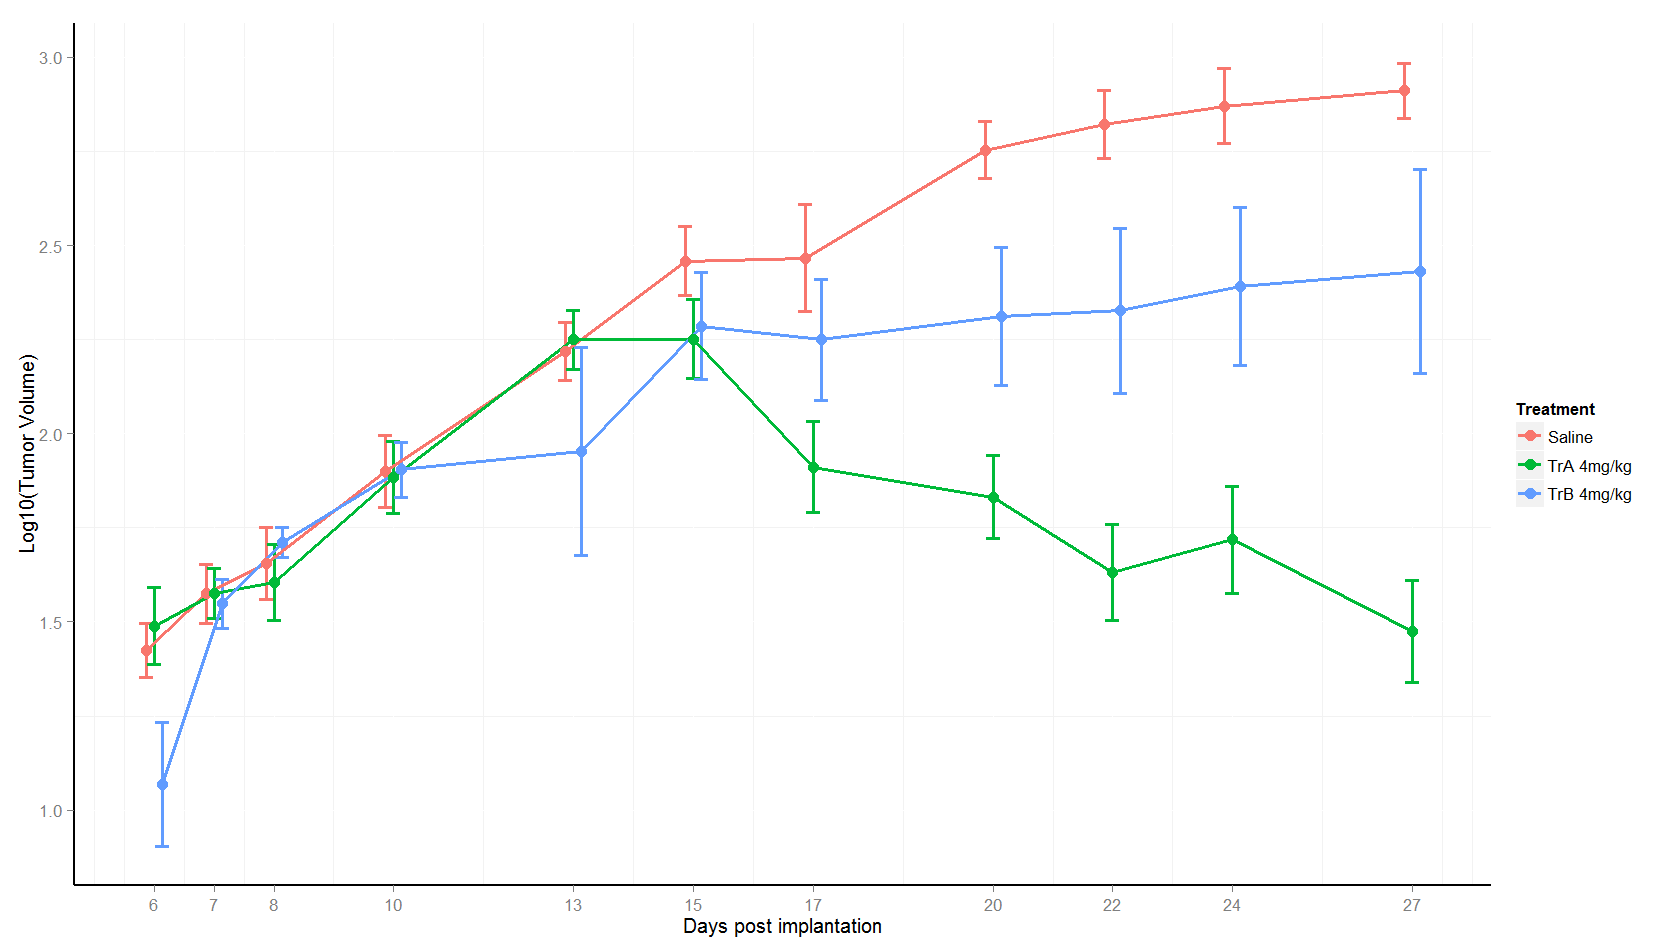
\includegraphics[width=\textwidth]{xenograph/figures/error_bars_log_LOCF_reduced_follow-up.png}
	\caption{Mean log$_{10}$-transformed tumour volume (mm$^3$) and standard errors for particular treatment lines over the follow-up after last-observation-carried-forward (LOCF) imputation.}
	\label{error_bars_log_LOCF_reduced_follow-up}
\end{figure}

Once therapeutic effect of Treatment A is clear regardless the data were considered in their raw or imputed form, the effect of Treatment B differs in both cases.
If the data is left unchanged, the Control and Treatment B outcomes do not differ from each other, indicating a lack of therapeutic effect from the treatment.
If the outcomes are compared on the data imputed with LOCF method both outcomes separate showing a treatment window between 15 and 27 days post implantation.
Imputation artificially increased separation between the Control and Treatment B group tumour volumes, such that the test shown the statistically significant effect from the therapy.
Therefore, imputation of the informed missing needs to be carefully considered as it may leads to faulty assessment of treatment effects.
It is not recommended for tumour xenograft studies.
The credit should be given to statistical methods which utilises a whole empirical evidence without a needs for data imputation.

\section{Statistical analysis}

The standard way of analysing the efficacy of a treatment is to establish whether there is a statistically significant difference between the treatment group and the control group.

Next we will introduce a series of statistical tests that can be applied to time-series data such as that reported by tumour xenograft experiments.
We will focus on measures of the efficacy of the TrA and TrB treatments over the control group.

We will both explore why common statistical tests may not be the best approach for this type of data, and introduce statistical tests that take all evidence into account when assessing treatment efficacy: permutation testing, and mixed-effect modelling.

\subsection{ANOVA}

A large proportion of (a subset of) historic xenograft were found to have used ANOVA or Kruskal-Wallis tests to analyse treatment efficacy \autocite{Heitjan:1993uw}.
There are multiple approaches that can be used when applying these tests to lognitudinal time-series.
Application of ANOVA requires the samples at each time point to be complete and to fulfil the statistical assumptions regarding the symmetry of distributions.
\begin{marginnoteblock}
	Normality of distribution is difficult to be assessed given the small sample size.
	Therefore, after \autocite{Heitjan:1993uw}, symmetry of distribution might be considered as a primary feature of normality.
\end{marginnoteblock}

The simplest method would be to examine the data at the final day with complete data.
\ldots
%The first animal drop out the study on day 15, which constitutes the last day for the (balanced) 1-way ANOVA with Treatment.
%Given the length of the follow-up (up to day 34) such an evidence is not considered to be relevant for a credible assessment of the treatment efficacy.

The next simplest method would be to apply ANOVA at each time point, testing for significance of the treatment at each discrete time, and so reporting a p-value for each.
% TODO Do some R code here
However, note that the type I error rate over the entire dataset is not 5\%.
This is because, with $n$ time points, we have $n$ chances to obtain a significant result purely by chance.
Therefore the overall chance of significance is much larger than 5\% -- the chance of at least one of the time points being significant just by chance is $1 - 0.95^n$.
\Cref{fig:multiple-significance} shows how the probability of finding at least one significant result by chance increases as the number of tests increases.

\begin{figure}
  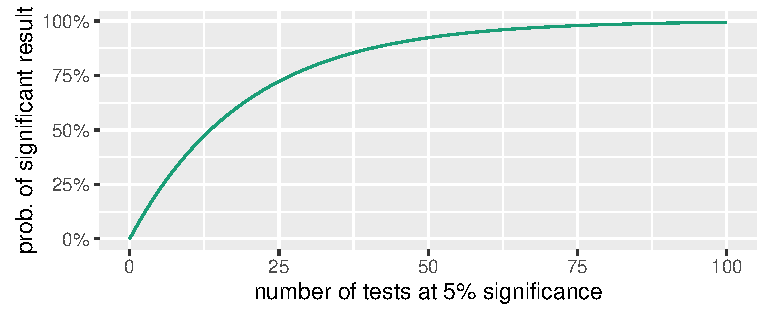
\includegraphics{xenograph/figures/multiple_significance.pdf}
  \caption{\ldots}
  \label{fig:multiple-significance}
\end{figure}

In order to correct for this \emph{multiple comparisons problem}, we could modify the significance level for each individual test.
There are multiple ways to do this, but one simple and conservative approach is to use the \textbf{Bonferroni correction}.
Using this correction, we set the significance level of each test to $\frac{0.05}{n}$.
However, this correction comes with the disadvantage of increasing the number of false negatives.

Other extensions to ANOVA might be considered.
\ldots

\subsection{Log-rank test}
The time-points when the tumours reached a certain end-point (e.g.\
doubled from the pre-treatment level) are compared with survival analysis tools.
The therapy is more effective if it prolongs significantly the time the end-point is reached.
Unfortunately, such an approach discards the tumour growth dynamics, and therefore cannot be considered as effective in helping to understand the underlying tumour biology, an important aspect in pre-clinical development.
It has also a limited applicability if sample tumours do not reach the end points over the follow-up period.

\subsection{Permutation-based test}
The alternative approach for the analysis of variance.

The permutation-base testing is widely applied as an alternative to classical null hypothesis tests.
The procedure relies on a series of repeated operations on the permuted sample data, resulting with a set of test statistics.
The proportion of outcomes which exceed the value acquired on the original (un-permuted) sample constitutes the significance of the difference between the groups \autocite{Ninness:2002ft}.
Therefore, the permutation-based tests are considered to be distribution- and assumption-free.
These tests can use different metrics to assess the group differences.
\textcite{PeresNeto:2001hz,Ludbrook:1998iv} show that permutation-based approach has a superior to classical approaches power once the sample size is insufficient or the statistical assumptions for `traditional' testing (e.g.\ t-, F-test) are violated.
Numerous versions of permutation tests were proposed to assess the tumour growth curve differences (e.g.\, \textcite{Koziol:1981gg,Rocchetti:1990bu}).
We adopt a relatively recent approach from \textcite{Elso:2004jp} to test the differences between the tumour growth curves in our pre-clinical \emph{in-vivo} experiments.
The particular steps of the test we apply is described in \cref{Appendix_Permutation_test}.
The presented permutation-based test has some important advantages in the analysis of pre-clinical tumour growth inhibition studies.
First of all, it does not require any particular statistical assumptions to be fulfilled.
Then, it is insensitive to missing data (no imputation required).
It allows for comparing evidence from multiple days, and by a proper weighting scheme, it gives more credit to the complete (representative) samples.
The procedure is implemented in the R statistical modelling packages \emph{statmod} \autocite{statmod:2013}.
Up to authors' best knowledge, the test has not been applied to test the difference between tumour curves in the xenograft experiments.
\Cref{permutation_test_table_log_whole_follow-up} delivers the test results for the whole sample (day 6--day 27).
To calculate the p-values $S=10^5$ permutations were used, and Holm's correction was applied to account for a potential multiple testing bias.

\begin{table}
	\centering
	\begin{tabular}{llrrr}
		\hline
		Group1     & Group2     & t-value & p-value & p-value (Holm) \\
		\hline
		Saline     & TrA 4mg/kg & 1.935   & 0.001   & 0.003          \\
		Saline     & TrB 4mg/kg & 0.743   & 0.157   & 0.314          \\
		TrA 4mg/kg & TrB 4mg/kg & -0.646  & 0.243   & 0.314          \\
		\hline
	\end{tabular}
	\caption{Permutation-based test outcome for log$_{10}$-transformed tumour volume (mm$^3$) differences between the treatment lines over a whole selected follow-up period.
		$S=10^5$ permutations were used to calculate the p-values.
	Holm's correction was applied to address the multiple testing bias.}
	\label{permutation_test_table_log_whole_follow-up}
\end{table}

To find the treatment effect window, the permutation test was carried out over different follow-up subsamples starting from day 6 onwards, and ending on day 27.
\Cref{p-values_log} delivers the resulting (Holm's corrected) p-values for the tumour inhibition differences observed for the treatment pairs.
Results show consistent and significant Treatment A effect.
The evidence from Treatment B is not significant on 0.05 level in none of the cases.
The difference between Treatment A and B effects are not significantly different either.
These two approaches work well once used together complementing their findings.
The example analysis was carried out with the R statistical computing language \autocite{rlang:2013}.

\begin{figure}
	\centering
	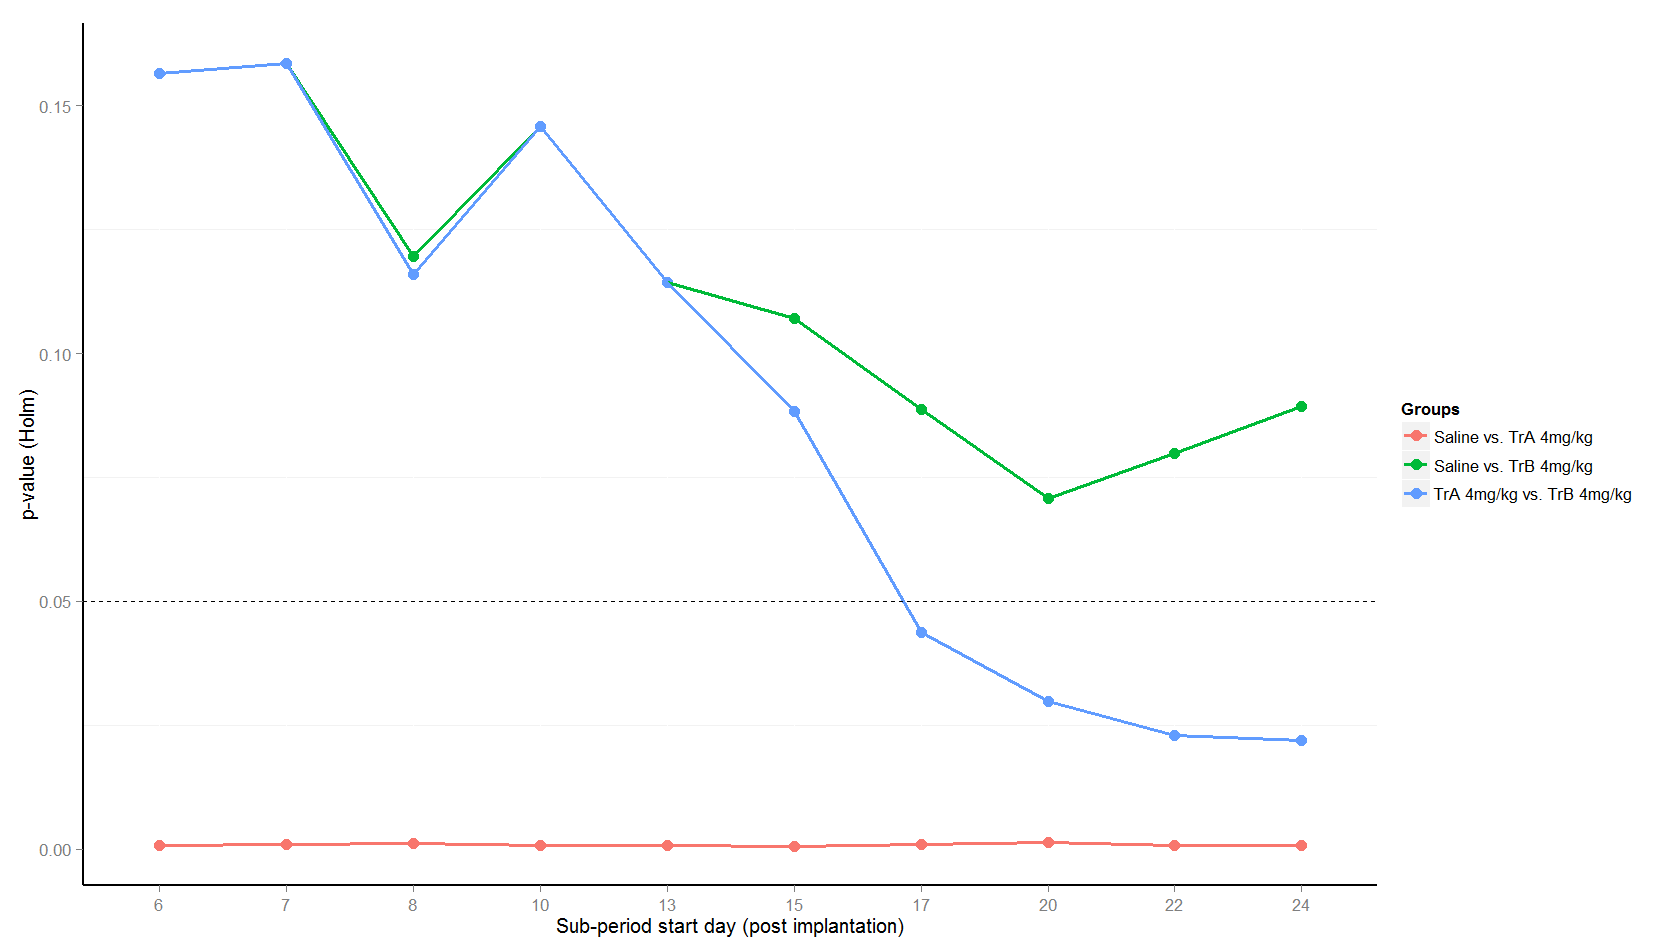
\includegraphics[width=\textwidth]{xenograph/figures/p-values_log.png}
	\caption{Adjusted (Holm's correction) p-values from the permutation test of the differences between log$_{10}$-transformed tumour volumes (mm$^3$) over sub-periods ending-up on Day 27.
		Starting days are on the horizontal axis.
		To calculate the p-values $S=10^5$ permutations were used.}
	\label{p-values_log}
\end{figure}


\subsection{Mixed-effect model}
The following skeleton of the mixed-effect model was used to assess the treatment efficacy \autocite{Laajala:2012kr,Demidenko:2010gn}:
\begin{align}
	\label{LME}
	\log_{10}\text{TV} = a_{1} + a_{2}\text{Tp} + a_{3}\text{Tr} + a_{4}\text{Tp : Tr} + (1|\text{No})
\end{align}
where:
\begin{itemize}
	\item `TV' is a tumour volume (mm$^3$)
	\item `Tp' readout time-point
	\item `Tr' stands for treatment line
	\item `No' is an tumour number.
\end{itemize}
Symbol `:' denotes the interaction between treatment and timepoint.
We consider two types of the \cref{LME}: with a linear time trend; and with repeated measurements.

\subsubsection{Model with linear time trend}
Within the \cref{LME} framework, consider time trend lines for two treatment groups:
\begin{align*}
	\text{Tr=0 (baseline)}&:\log_{10}\text{TV} = a_{1} + a_{2}\text{Tp} \\
	\text{Tr=1 (investigated)}&:\log_{10}\text{TV} = a_{1} + a_{3} + (a_{2}+ a_{4})\text{Tp}.
\end{align*}
In the investigated trend line parameters $a_{3}$ and $a_{4}$ affect the intercept and slope parameters of the baseline model, respectively.
These parameters will be used in the assessment of the treatment effect resulting from the investigated therapy.
In particular, after \autocite{Laajala:2012kr}, the offset parameter $a_{3}$ represents the changes in the horizontal base level profiles, and the interaction term parameter $a_{4}$ the change in the time trend.
The latter effect will be expressed as the effective growth inhibition rate (GIR):
\begin{align}
	\text{GIR}:= 100 \times \left|\frac{a_{4}}{a_{2}}\right| \%
\end{align}
will be used as a primary measure of the treatment effect from the investigated therapy line.


The model was applied to the experimental data.
\Cref{LME_trend_TrA_TrB_baseline_Saline} provides the \cref{LME} fixed effect outcomes if the efficacy of the treatment lines is considered with respect to the Saline.
On a log$_{10}$-basis, the Tumour Volume in the Saline group increases by 0.171 on average per day.
The baseline slope gets (on average) reduced by 0.151 ($p<0.001$) and 0.027 (p=0.203) in the TrA and TrB groups, respectively, but only the first effect remains significant on the 0.05 level.
These results translate into 88.2\% growth inhibition rate in TrA line, where usually at least 55\% reduction is considered as a significant improvement \autocite{Cheng:2010bp}.

\Cref{LME_trend_TrA_baseline_TrB} provides the \cref{LME} fixed effect outcomes if the efficacy of TrA line is considered with respect to the TrB.
The average Tumour Volume growth in the TrB (baseline) group is 0.145 ($p<0.001$) on the log$_{10}$ scale.
The TrA (investigated) therapy reduces significantly the baseline growth by 0.124 ($p<0.001$) which translates into a GIR=85.5\%.

Treatment TrA significantly improves over both the Saline and TrB groups in terms of the linear Tumour Volume growth reduction expressed by the growth inhibition rates of at least of 85\%.
Treatment effect within TrB group over the Saline is not statistically significant at 5\% level.

\begin{table}
	\centering
	\small
	\begin{tabular}{lccccc}
		\hline
		                              & Coefficient & Std Error & df    & t-value & p-value \\
		\hline
		(Intercept)                   & 1.265       & 0.106     & 89.8  & 11.981  & 0.000   \\
		time-point                     & 0.171       & 0.015     & 207.2 & 11.674  & 0.000   \\
		TreatmentTrA 4mg/kg           & 0.444       & 0.149     & 89.2  & 2.979   & 0.004   \\
		TreatmentTrB 4mg/kg           & -0.050      & 0.149     & 89.6  & -0.334  & 0.739   \\
		time-point:TreatmentTrA 4mg/kg & -0.151      & 0.021     & 208.5 & -7.271  & 0.000   \\
		time-point:TreatmentTrB 4mg/kg & -0.027      & 0.021     & 209.8 & -1.277  & 0.203   \\
		\hline
	\end{tabular}
	\caption{Mixed effect model with linear trend fixed effect parameters with diagnostics.
	The baseline treatment group is the control one (Saline).}
	\label{LME_trend_TrA_TrB_baseline_Saline}
\end{table}

\begin{table}
	\centering
	\small
	\begin{tabular}{lccccc}
		\hline
		                              & Coefficient & Std Error & df    & t-value & p-value \\
		\hline
		(Intercept)                   & 1.265       & 0.092     & 60.9  & 13.799  & 0.000   \\
		time-point                     & 0.171       & 0.013     & 139.7 & 13.356  & 0.000   \\
		TreatmentTrA 4mg/kg           & 0.444       & 0.130     & 60.5  & 3.426   & 0.001   \\
		time-point:TreatmentTrA 4mg/kg & -0.151      & 0.018     & 140.6 & -8.316  & 0.000   \\
		\hline
	\end{tabular}
	\caption{Mixed effect model with linear trend: fixed effect parameters with diagnostics.
	The baseline treatment group is TrA 4mg/kg.}
	\label{LME_trend_TrA_basline_Saline}
\end{table}

\begin{table}
	\centering
	\small
	\begin{tabular}{lccccc}
		\hline
		                              & Coefficient & Std Error & df    & t-value & p-value \\
		\hline
		(Intercept)                   & 1.263       & 0.107     & 54.7  & 11.854  & 0.000   \\
		time-point                     & 0.172       & 0.014     & 137.3 & 11.853  & 0.000   \\
		TreatmentTrB 4mg/kg           & -0.048      & 0.151     & 54.6  & -0.320  & 0.750   \\
		time-point:TreatmentTrB 4mg/kg & -0.027      & 0.021     & 139.0 & -1.315  & 0.191   \\
		\hline
	\end{tabular}
	\caption{Mixed effect model with linear trend: fixed effect parameters with diagnostics.
	The baseline treatment group is TrA 4mg/kg.}
	\label{LME_trend_TrB_basline_Saline}
\end{table}


\begin{table}
	\centering
	\small
	\begin{tabular}{lccccc}
		\hline
		                              & Coefficient & Std Error & df    & t-value & p-value \\
		\hline
		(Intercept)                   & 1.215       & 0.117     & 63.5  & 10.353  & 0.000   \\
		time-point                     & 0.145       & 0.017     & 140.5 & 8.562   & 0.000   \\
		TreatmentTrA 4mg/kg           & 0.494       & 0.166     & 63.2  & 2.982   & 0.004   \\
		time-point:TreatmentTrA 4mg/kg & -0.124      & 0.024     & 139.9 & -5.253  & 0.000   \\
		\hline
	\end{tabular}
	\caption{Mixed effect model with linear trend fixed effect parameters with diagnostics.
	The baseline treatment group is TrB 4mg/kg.}
	\label{LME_trend_TrA_baseline_TrB}
\end{table}

\subsubsection{Model with repeated measurements}
If time-point Tp in \cref{LME} is considered as a factor/class, the model assesses the therapy effectiveness for each day with respect to the baseline treatment outcomes at a particular time-point after tumour cells implantation.
Such specification allows for a precise assessment of the treatments effects for each follow-up day and (if available) an identification of a `treatment window', a period where the drug was effective over the baseline group.
These results complement the outcomes of the trend analysis.

\Cref{LME_factor_TrA_TrB_baseline_Saline} provides the fixed-effect model outcomes if the Saline group is considered as a baseline treatment, with reference time-point at day 6.
We mainly concentrate on the interaction parameter values ($\alpha_{4}$), which allow for assessment of therapeutic effects for each treatment line and time-point.
The p-values suggest that the TrA shows its efficacy over the Saline from day 17 onwards at the 5\% significance.
TrB line is not effective over the Saline.
These parameter values reflect the differences between the (log$_{10}$-transformed) Tumour Volume model least-squares means estimated at baseline and investigated time-points for the control and investigated treatment lines:
\begin{align}
	\alpha_{4} = TV_{2,2} - TV_{1,2} - (TV_{2,1} - TV_{1,1})
\end{align}
where:
\begin{table}
	\centering
	\small
	\begin{tabular}{c|cc}
		                & Tp baseline & Tp investigated \\
		\hline
		Tr baseline     & $TV_{1,1}$  & $TV_{1,2}$      \\
		Tr investigated & $TV_{2,1}$  & $TV_{2,2}$      \\
	\end{tabular}
	\caption{Selected least-squares $\log_{10}$ transformed Tumour Volume ($TV$) mean values inferred from the \cref{LME}.}
	\label{effects}
\end{table}
The least-squares means for the model where Saline is considered as a baseline are provided in \cref{effects_LME_factor_TrA_TrB_baseline_Saline}.
For example, the treatment TrA for day 17 interaction term parameter value of $-0.620$ (see corresponding \cref{LME_factor_TrA_TrB_baseline_Saline}) equals $1.911 - 2.466 - ( 1.489 - 1.424)$.
Such a value suggests a greater by 0.62 reduction of the log$_{10}$ Tumour Volume at the investigated time-point compared to the baseline.
If values in \cref{effects} are considered as log$_{10}$ values of mean tumour volumes:
\begin{align*}
	\log_{10}TV_{2,2} - \log_{10}TV_{1,2} - (\log_{10}TV_{2,1} - \log_{10}TV_{1,1}) = \alpha_{4}
\end{align*}
then the above align translates into:
\begin{align}
	\label{effect_size}
	\frac{TV_{2,2}\;TV_{1,1}}{TV_{1,2}\;TV_{2,1}} = 10^{\alpha_{4}}.
\end{align}
\Cref{effect_size} allows for interpretation of $\alpha_{4}$ as of the relative change of T/C measure observed at the investigated time-point to the baseline one.
With that respect the observed effect on day 17 from TrA equals to 24\%.


A more straightforward assessment of the treatment effect at the investigated time-point (Tp investigated) can be acquired from the least-squares means as:
\begin{align}
	100\times \left(1-\frac{TV_{2,2}}{TV_{1,2}}\right) \%,
\end{align}
which in the case of day 17 for treatment A (Tr A) equals to $22.5\% (=1 - 1.911/2.466)$ on the log$_{10}$ scale, and this measure is suggested to be used.
For the following days, the effects are $33.4\%$ (day 20), $42.9\%$ (day 22), $33.7\%$ (day 24), and $51.7\%$ (day 27).
Similar analysis can be carried out for the model where the efficacy of TrA is considered with respect to TrB, see \cref{LME_factor_TrA_baseline_TrB,effects_LME_factor_TrA_baseline_TrB}.


\newpage
\begin{table}
	\centering
	\small
	\begin{tabular}{lccccc}
		\hline
		                                & Coefficient & Std Error & df    & t-value & p-value \\
		\hline
		(Intercept)                     & 1.424       & 0.132     & 142.7 & 10.765  & 0.000   \\
		time-point7                      & 0.151       & 0.166     & 173.5 & 0.908   & 0.365   \\
		time-point8                      & 0.232       & 0.166     & 173.5 & 1.397   & 0.164   \\
		time-point10                     & 0.476       & 0.166     & 173.5 & 2.861   & 0.005   \\
		time-point13                     & 0.795       & 0.166     & 173.5 & 4.780   & 0.000   \\
		time-point15                     & 1.034       & 0.166     & 173.5 & 6.219   & 0.000   \\
		time-point17                     & 1.042       & 0.166     & 173.5 & 6.269   & 0.000   \\
		time-point20                     & 1.341       & 0.173     & 174.5 & 7.765   & 0.000   \\
		time-point22                     & 1.418       & 0.173     & 174.5 & 8.215   & 0.000   \\
		time-point24                     & 1.388       & 0.206     & 177.2 & 6.728   & 0.000   \\
		time-point27                     & 1.424       & 0.229     & 178.1 & 6.215   & 0.000   \\
		TreatmentTrA 4mg/kg             & 0.065       & 0.187     & 142.7 & 0.348   & 0.728   \\
		TreatmentTrB 4mg/kg             & -0.356      & 0.187     & 142.7 & -1.901  & 0.059   \\
		time-point7:TreatmentTrA 4mg/kg  & -0.064      & 0.235     & 173.5 & -0.271  & 0.787   \\
		time-point8:TreatmentTrA 4mg/kg  & -0.116      & 0.235     & 173.5 & -0.494  & 0.622   \\
		time-point10:TreatmentTrA 4mg/kg & -0.081      & 0.235     & 173.5 & -0.343  & 0.732   \\
		time-point13:TreatmentTrA 4mg/kg & -0.034      & 0.235     & 173.5 & -0.144  & 0.886   \\
		time-point15:TreatmentTrA 4mg/kg & -0.271      & 0.235     & 173.5 & -1.154  & 0.250   \\
		time-point17:TreatmentTrA 4mg/kg & -0.620      & 0.235     & 173.5 & -2.638  & 0.009   \\
		time-point20:TreatmentTrA 4mg/kg & -0.989      & 0.244     & 174.5 & -4.051  & 0.000   \\
		time-point22:TreatmentTrA 4mg/kg & -1.284      & 0.258     & 175.7 & -4.980  & 0.000   \\
		time-point24:TreatmentTrA 4mg/kg & -1.013      & 0.292     & 177.3 & -3.469  & 0.001   \\
		time-point27:TreatmentTrA 4mg/kg & -1.536      & 0.308     & 177.8 & -4.981  & 0.000   \\
		time-point7:TreatmentTrB 4mg/kg  & 0.329       & 0.235     & 173.5 & 1.399   & 0.164   \\
		time-point8:TreatmentTrB 4mg/kg  & 0.411       & 0.235     & 173.5 & 1.746   & 0.083   \\
		time-point10:TreatmentTrB 4mg/kg & 0.360       & 0.235     & 173.5 & 1.532   & 0.127   \\
		time-point13:TreatmentTrB 4mg/kg & 0.090       & 0.235     & 173.5 & 0.382   & 0.703   \\
		time-point15:TreatmentTrB 4mg/kg & 0.184       & 0.235     & 173.5 & 0.782   & 0.435   \\
		time-point17:TreatmentTrB 4mg/kg & 0.187       & 0.240     & 174.2 & 0.779   & 0.437   \\
		time-point20:TreatmentTrB 4mg/kg & -0.071      & 0.250     & 175.2 & -0.283  & 0.777   \\
		time-point22:TreatmentTrB 4mg/kg & -0.021      & 0.258     & 175.8 & -0.081  & 0.935   \\
		time-point24:TreatmentTrB 4mg/kg & 0.113       & 0.282     & 177.1 & 0.400   & 0.690   \\
		time-point27:TreatmentTrB 4mg/kg & -0.036      & 0.324     & 178.2 & -0.110  & 0.912   \\
		\hline
	\end{tabular}
	\caption{Linear mixed effect model fixed effect parameters with diagnostics.
	The baseline treatment group is the control one (Saline) with reference time-point on day 6.}
	\label{LME_factor_TrA_TrB_baseline_Saline}
\end{table}


\begin{table}
	\centering
	\small
	\begin{tabular}{lccccc}
		\hline
		                                & Coefficient & Std Error & df    & t-value & p-value \\
		\hline
		(Intercept)                     & 1.424       & 0.105     & 80.3  & 13.514  & 0.000   \\
		time-point7                      & 0.151       & 0.127     & 117.0 & 1.188   & 0.237   \\
		time-point8                      & 0.232       & 0.127     & 117.0 & 1.829   & 0.070   \\
		time-point10                     & 0.476       & 0.127     & 117.0 & 3.745   & 0.000   \\
		time-point13                     & 0.795       & 0.127     & 117.0 & 6.258   & 0.000   \\
		time-point15                     & 1.034       & 0.127     & 117.0 & 8.141   & 0.000   \\
		time-point17                     & 1.042       & 0.127     & 117.0 & 8.207   & 0.000   \\
		time-point20                     & 1.343       & 0.132     & 117.6 & 10.182  & 0.000   \\
		time-point22                     & 1.421       & 0.132     & 117.6 & 10.770  & 0.000   \\
		time-point24                     & 1.396       & 0.158     & 119.0 & 8.842   & 0.000   \\
		time-point27                     & 1.434       & 0.175     & 119.5 & 8.179   & 0.000   \\
		TreatmentTrA 4mg/kg             & 0.065       & 0.149     & 80.3  & 0.437   & 0.663   \\
		time-point7:TreatmentTrA 4mg/kg  & -0.064      & 0.180     & 117.0 & -0.355  & 0.723   \\
		time-point8:TreatmentTrA 4mg/kg  & -0.116      & 0.180     & 117.0 & -0.647  & 0.519   \\
		time-point10:TreatmentTrA 4mg/kg & -0.081      & 0.180     & 117.0 & -0.449  & 0.655   \\
		time-point13:TreatmentTrA 4mg/kg & -0.034      & 0.180     & 117.0 & -0.188  & 0.851   \\
		time-point15:TreatmentTrA 4mg/kg & -0.271      & 0.180     & 117.0 & -1.511  & 0.133   \\
		time-point17:TreatmentTrA 4mg/kg & -0.620      & 0.180     & 117.0 & -3.453  & 0.001   \\
		time-point20:TreatmentTrA 4mg/kg & -0.991      & 0.187     & 117.6 & -5.314  & 0.000   \\
		time-point22:TreatmentTrA 4mg/kg & -1.291      & 0.197     & 118.2 & -6.548  & 0.000   \\
		time-point24:TreatmentTrA 4mg/kg & -1.028      & 0.223     & 119.1 & -4.603  & 0.000   \\
		time-point27:TreatmentTrA 4mg/kg & -1.554      & 0.236     & 119.3 & -6.586  & 0.000   \\
		\hline
	\end{tabular}
	\caption{Linear mixed effect model: fixed effect parameters with diagnostics.
	The baseline treatment group is the control one (Saline).}
	\label{LME_factor_TrA_baseline_Saline}
\end{table}


\begin{table}
	\centering
	\small
	\begin{tabular}{lccccc}
		\hline
		                                & Coefficient & Std Error & df    & t-value & p-value \\
		\hline
		(Intercept)                     & 1.424       & 0.141     & 104.2 & 10.108  & 0.000   \\
		time-point7                      & 0.151       & 0.181     & 115.3 & 0.832   & 0.407   \\
		time-point8                      & 0.232       & 0.181     & 115.3 & 1.280   & 0.203   \\
		time-point10                     & 0.476       & 0.181     & 115.3 & 2.622   & 0.010   \\
		time-point13                     & 0.795       & 0.181     & 115.3 & 4.381   & 0.000   \\
		time-point15                     & 1.034       & 0.181     & 115.3 & 5.700   & 0.000   \\
		time-point17                     & 1.042       & 0.181     & 115.3 & 5.746   & 0.000   \\
		time-point20                     & 1.339       & 0.188     & 116.1 & 7.108   & 0.000   \\
		time-point22                     & 1.416       & 0.188     & 116.1 & 7.520   & 0.000   \\
		time-point24                     & 1.383       & 0.225     & 118.2 & 6.147   & 0.000   \\
		time-point27                     & 1.416       & 0.250     & 118.9 & 5.672   & 0.000   \\
		TreatmentTrB 4mg/kg             & -0.356      & 0.199     & 104.2 & -1.785  & 0.077   \\
		time-point7:TreatmentTrB 4mg/kg  & 0.329       & 0.257     & 115.3 & 1.282   & 0.202   \\
		time-point8:TreatmentTrB 4mg/kg  & 0.411       & 0.257     & 115.3 & 1.601   & 0.112   \\
		time-point10:TreatmentTrB 4mg/kg & 0.360       & 0.257     & 115.3 & 1.405   & 0.163   \\
		time-point13:TreatmentTrB 4mg/kg & 0.090       & 0.257     & 115.3 & 0.351   & 0.727   \\
		time-point15:TreatmentTrB 4mg/kg & 0.184       & 0.257     & 115.3 & 0.717   & 0.475   \\
		time-point17:TreatmentTrB 4mg/kg & 0.188       & 0.262     & 115.8 & 0.717   & 0.475   \\
		time-point20:TreatmentTrB 4mg/kg & -0.069      & 0.273     & 116.7 & -0.253  & 0.801   \\
		time-point22:TreatmentTrB 4mg/kg & -0.015      & 0.281     & 117.1 & -0.054  & 0.957   \\
		time-point24:TreatmentTrB 4mg/kg & 0.122       & 0.307     & 118.1 & 0.398   & 0.691   \\
		time-point27:TreatmentTrB 4mg/kg & -0.027      & 0.353     & 119.0 & -0.076  & 0.939   \\
		\hline
	\end{tabular}
	\caption{Linear mixed effect model: fixed effect parameters with diagnostics.
	The baseline treatment group is the control one (Saline).}
	\label{LME_factor_TrB_baseline_Saline}
\end{table}

\newpage
\begin{table}
	\centering
	\small
	\begin{tabular}{lccccc}
		\hline
		                                & Coefficient & Std Error & df    & t-value & p-value \\
		\hline
		(Intercept)                     & 1.068       & 0.147     & 94.4  & 7.257   & 0.000   \\
		time-point7                      & 0.480       & 0.185     & 114.6 & 2.597   & 0.011   \\
		time-point8                      & 0.643       & 0.185     & 114.6 & 3.479   & 0.001   \\
		time-point10                     & 0.836       & 0.185     & 114.6 & 4.525   & 0.000   \\
		time-point13                     & 0.885       & 0.185     & 114.6 & 4.788   & 0.000   \\
		time-point15                     & 1.218       & 0.185     & 114.6 & 6.592   & 0.000   \\
		time-point17                     & 1.229       & 0.192     & 115.4 & 6.405   & 0.000   \\
		time-point20                     & 1.270       & 0.201     & 116.2 & 6.319   & 0.000   \\
		time-point22                     & 1.397       & 0.213     & 116.8 & 6.563   & 0.000   \\
		time-point24                     & 1.501       & 0.213     & 116.8 & 7.049   & 0.000   \\
		time-point27                     & 1.388       & 0.255     & 117.8 & 5.450   & 0.000   \\
		TreatmentTrA 4mg/kg             & 0.421       & 0.208     & 94.4  & 2.021   & 0.046   \\
		time-point7:TreatmentTrA 4mg/kg  & -0.393      & 0.261     & 114.6 & -1.503  & 0.136   \\
		time-point8:TreatmentTrA 4mg/kg  & -0.527      & 0.261     & 114.6 & -2.016  & 0.046   \\
		time-point10:TreatmentTrA 4mg/kg & -0.441      & 0.261     & 114.6 & -1.687  & 0.094   \\
		time-point13:TreatmentTrA 4mg/kg & -0.124      & 0.261     & 114.6 & -0.474  & 0.637   \\
		time-point15:TreatmentTrA 4mg/kg & -0.455      & 0.261     & 114.6 & -1.743  & 0.084   \\
		time-point17:TreatmentTrA 4mg/kg & -0.807      & 0.266     & 115.1 & -3.029  & 0.003   \\
		time-point20:TreatmentTrA 4mg/kg & -0.918      & 0.278     & 115.7 & -3.305  & 0.001   \\
		time-point22:TreatmentTrA 4mg/kg & -1.263      & 0.301     & 116.7 & -4.196  & 0.000   \\
		time-point24:TreatmentTrA 4mg/kg & -1.126      & 0.313     & 117.0 & -3.596  & 0.000   \\
		time-point27:TreatmentTrA 4mg/kg & -1.501      & 0.343     & 117.5 & -4.378  & 0.000   \\
		\hline
	\end{tabular}
	\caption{Linear mixed effect model fixed effect parameters with diagnostics.
	The baseline treatment group is TrB 4mg/kg with reference time-point on day 6.}
	\label{LME_factor_TrA_baseline_TrB}
\end{table}

\begin{figure}
	\centering
	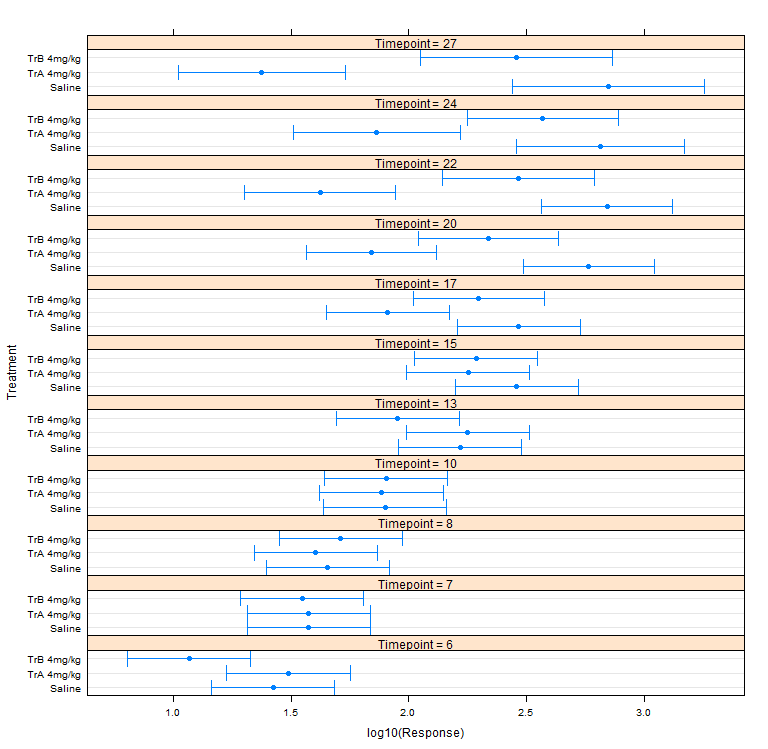
\includegraphics[width=\textwidth]{xenograph/figures/effects_LME_factor1.png}
	\caption{Least squares means with 95\% confidence intervals for each treatment line and time-point after cancer cells implantation.}
	\label{effects_LME_factor}
\end{figure}

\newpage
\begin{table}
	\centering
	\begin{tabular}{rllrrrrr}
		\hline
		   & Treatment  & time-point & lsmean & SE    & df      & lower.CL & upper.CL \\
		\hline
		1  & Saline     & 6         & 1.424  & 0.132 & 141.771 & 1.162    & 1.685    \\
		2  & TrA 4mg/kg & 6         & 1.489  & 0.132 & 141.771 & 1.227    & 1.750    \\
		3  & TrB 4mg/kg & 6         & 1.068  & 0.132 & 141.771 & 0.807    & 1.330    \\
		4  & Saline     & 7         & 1.575  & 0.132 & 141.771 & 1.313    & 1.836    \\
		5  & TrA 4mg/kg & 7         & 1.576  & 0.132 & 141.771 & 1.315    & 1.837    \\
		6  & TrB 4mg/kg & 7         & 1.548  & 0.132 & 141.771 & 1.287    & 1.810    \\
		7  & Saline     & 8         & 1.656  & 0.132 & 141.771 & 1.395    & 1.918    \\
		8  & TrA 4mg/kg & 8         & 1.605  & 0.132 & 141.771 & 1.343    & 1.866    \\
		9  & TrB 4mg/kg & 8         & 1.711  & 0.132 & 141.771 & 1.450    & 1.973    \\
		10 & Saline     & 10        & 1.899  & 0.132 & 141.771 & 1.638    & 2.161    \\
		11 & TrA 4mg/kg & 10        & 1.884  & 0.132 & 141.771 & 1.623    & 2.145    \\
		12 & TrB 4mg/kg & 10        & 1.904  & 0.132 & 141.771 & 1.643    & 2.166    \\
		13 & Saline     & 13        & 2.219  & 0.132 & 141.771 & 1.957    & 2.480    \\
		14 & TrA 4mg/kg & 13        & 2.250  & 0.132 & 141.771 & 1.988    & 2.511    \\
		15 & TrB 4mg/kg & 13        & 1.953  & 0.132 & 141.771 & 1.692    & 2.214    \\
		16 & Saline     & 15        & 2.458  & 0.132 & 141.771 & 2.196    & 2.719    \\
		17 & TrA 4mg/kg & 15        & 2.252  & 0.132 & 141.771 & 1.990    & 2.513    \\
		18 & TrB 4mg/kg & 15        & 2.286  & 0.132 & 141.771 & 2.025    & 2.548    \\
		19 & Saline     & 17        & 2.466  & 0.132 & 141.771 & 2.205    & 2.728    \\
		20 & TrA 4mg/kg & 17        & 1.911  & 0.132 & 141.771 & 1.650    & 2.173    \\
		21 & TrB 4mg/kg & 17        & 2.297  & 0.140 & 152.790 & 2.020    & 2.575    \\
		22 & Saline     & 20        & 2.765  & 0.140 & 153.087 & 2.487    & 3.042    \\
		23 & TrA 4mg/kg & 20        & 1.841  & 0.140 & 153.087 & 1.564    & 2.118    \\
		24 & TrB 4mg/kg & 20        & 2.338  & 0.150 & 164.207 & 2.041    & 2.635    \\
		25 & Saline     & 22        & 2.842  & 0.140 & 153.087 & 2.565    & 3.119    \\
		26 & TrA 4mg/kg & 22        & 1.623  & 0.163 & 175.691 & 1.302    & 1.945    \\
		27 & TrB 4mg/kg & 22        & 2.466  & 0.163 & 175.303 & 2.144    & 2.788    \\
		28 & Saline     & 24        & 2.812  & 0.180 & 185.452 & 2.456    & 3.168    \\
		29 & TrA 4mg/kg & 24        & 1.865  & 0.180 & 185.230 & 1.508    & 2.221    \\
		30 & TrB 4mg/kg & 24        & 2.569  & 0.163 & 175.303 & 2.247    & 2.891    \\
		31 & Saline     & 27        & 2.848  & 0.206 & 191.963 & 2.441    & 3.254    \\
		32 & TrA 4mg/kg & 27        & 1.377  & 0.180 & 185.230 & 1.020    & 1.733    \\
		33 & TrB 4mg/kg & 27        & 2.456  & 0.206 & 191.832 & 2.049    & 2.863    \\
		\hline
	\end{tabular}
	\caption{Least squares means with 95\% confidence intervals for each treatment line and time-point after cancer cells implantation.}
	\label{effects_LME_factor_TrA_TrB_baseline_Saline}
\end{table}


\begin{table}
	\centering
	\begin{tabular}{rllrrrrr}
		\hline
		   & Treatment  & time-point & lsmean & SE    & df      & lower.CL & upper.CL \\
		\hline
		1  & TrB 4mg/kg & 6         & 1.068  & 0.147 & 93.172  & 0.776    & 1.360    \\
		2  & TrA 4mg/kg & 6         & 1.489  & 0.147 & 93.172  & 1.197    & 1.781    \\
		3  & TrB 4mg/kg & 7         & 1.548  & 0.147 & 93.172  & 1.256    & 1.840    \\
		4  & TrA 4mg/kg & 7         & 1.576  & 0.147 & 93.172  & 1.284    & 1.868    \\
		5  & TrB 4mg/kg & 8         & 1.711  & 0.147 & 93.172  & 1.419    & 2.003    \\
		6  & TrA 4mg/kg & 8         & 1.605  & 0.147 & 93.172  & 1.313    & 1.897    \\
		7  & TrB 4mg/kg & 10        & 1.904  & 0.147 & 93.172  & 1.612    & 2.197    \\
		8  & TrA 4mg/kg & 10        & 1.884  & 0.147 & 93.172  & 1.592    & 2.176    \\
		9  & TrB 4mg/kg & 13        & 1.953  & 0.147 & 93.172  & 1.661    & 2.245    \\
		10 & TrA 4mg/kg & 13        & 2.250  & 0.147 & 93.172  & 1.958    & 2.542    \\
		11 & TrB 4mg/kg & 15        & 2.286  & 0.147 & 93.172  & 1.994    & 2.579    \\
		12 & TrA 4mg/kg & 15        & 2.252  & 0.147 & 93.172  & 1.959    & 2.544    \\
		13 & TrB 4mg/kg & 17        & 2.297  & 0.156 & 100.499 & 1.988    & 2.607    \\
		14 & TrA 4mg/kg & 17        & 1.911  & 0.147 & 93.172  & 1.619    & 2.203    \\
		15 & TrB 4mg/kg & 20        & 2.338  & 0.167 & 108.103 & 2.006    & 2.670    \\
		16 & TrA 4mg/kg & 20        & 1.841  & 0.156 & 100.692 & 1.531    & 2.150    \\
		17 & TrB 4mg/kg & 22        & 2.465  & 0.182 & 115.505 & 2.106    & 2.825    \\
		18 & TrA 4mg/kg & 22        & 1.623  & 0.181 & 115.759 & 1.264    & 1.983    \\
		19 & TrB 4mg/kg & 24        & 2.569  & 0.182 & 115.505 & 2.209    & 2.929    \\
		20 & TrA 4mg/kg & 24        & 1.864  & 0.201 & 122.135 & 1.466    & 2.262    \\
		21 & TrB 4mg/kg & 27        & 2.456  & 0.230 & 126.553 & 2.002    & 2.910    \\
		22 & TrA 4mg/kg & 27        & 1.376  & 0.201 & 122.135 & 0.979    & 1.774    \\
		\hline
	\end{tabular}
	\caption{Least squares means with 95\% confidence intervals for each treatment line and time-point after cancer cells implantation.}
	\label{effects_LME_factor_TrA_baseline_TrB}
\end{table}


\newpage
\subsection{LOESS}
The approach was originally proposed and further developed by \textcite{Cleveland:1979kf,Cleveland:1988de}.
It derives from LOWESS (\emph{LOcally WEighted Scatterplot Smoothing}) approach and corresponds to non-parametric regression methodology which relies on locally weighted regression to smooth the data \autocite{Cleveland:1981fm}.
The approach relies on a k-neighbor least-squares regression fits carried for each follow-up time-point.
The smoothing granularity is controlled by user-defined \emph{smoothing parameter}.
Particular steps of the LOESS algorithm are described in \cref{Appendix_LOESS}.
For the pre-clinical tumour growth inhibition studies, the LOESS approach allows for aggregation of the group trajectories into a smoothed trend line, tackling potential non-linearities of the tumour growth paths.
It helps to moderate an influence of the outliers and informed missing data, which is particularly important given a small sample nature of the experiments.
Precision of the smoothing can be assessed with 95\% confidence interval.
\textcite{Moses:1992dh} applied LOESS approach to analyse the animal growth curves.
We adapt it for the analysis of tumour growth data.
The resulting curve provides a visual assessment of the deterministic part of the data variation.
The separation between LOESS curves for treatment lines and their confidence interval bands may serve as an indication of possible treatment effects.
To deliver robust and representative results fairly large and dense datasets are required.
The method does not produce an accompanying closed-form mathematical formula (regression model) for the resulting curve.
It comes within the default \emph{stats} R package distribution, but is also available in majority of standard statistical packages available on the market.


\Cref{loess_trajectories_log_reduced_follow-up} provides results for the LOESS fit within each treatment line, together with 95\% confidence intervals.
The smoothing parameter was fixed at a default 0.75 level.
The tumour response patterns are more clear now.
For both treatments and Control the LOESS fits start separating from day 13 onwards.
However, only Treatment A shows on a strong therapeutic effect.
The difference for that group becomes statistically significant from day 15 onwards, where the confidence intervals do not overlap each other.
Response from Treatment B is mixed.
There are two groups of animals where one of them manifests in a shrinking tumour volume, and responds to the treatment.
The other one does not respond and tumour continues to grow roughly in line with the Control group pattern.
The LOESS curves still shows some separation but given that the confidence interval overlaps with Control one, the observed therapeutic effect cannot be considered statistically significant.
Application of permutation-based test solves that issue.

\begin{figure}
	\centering
	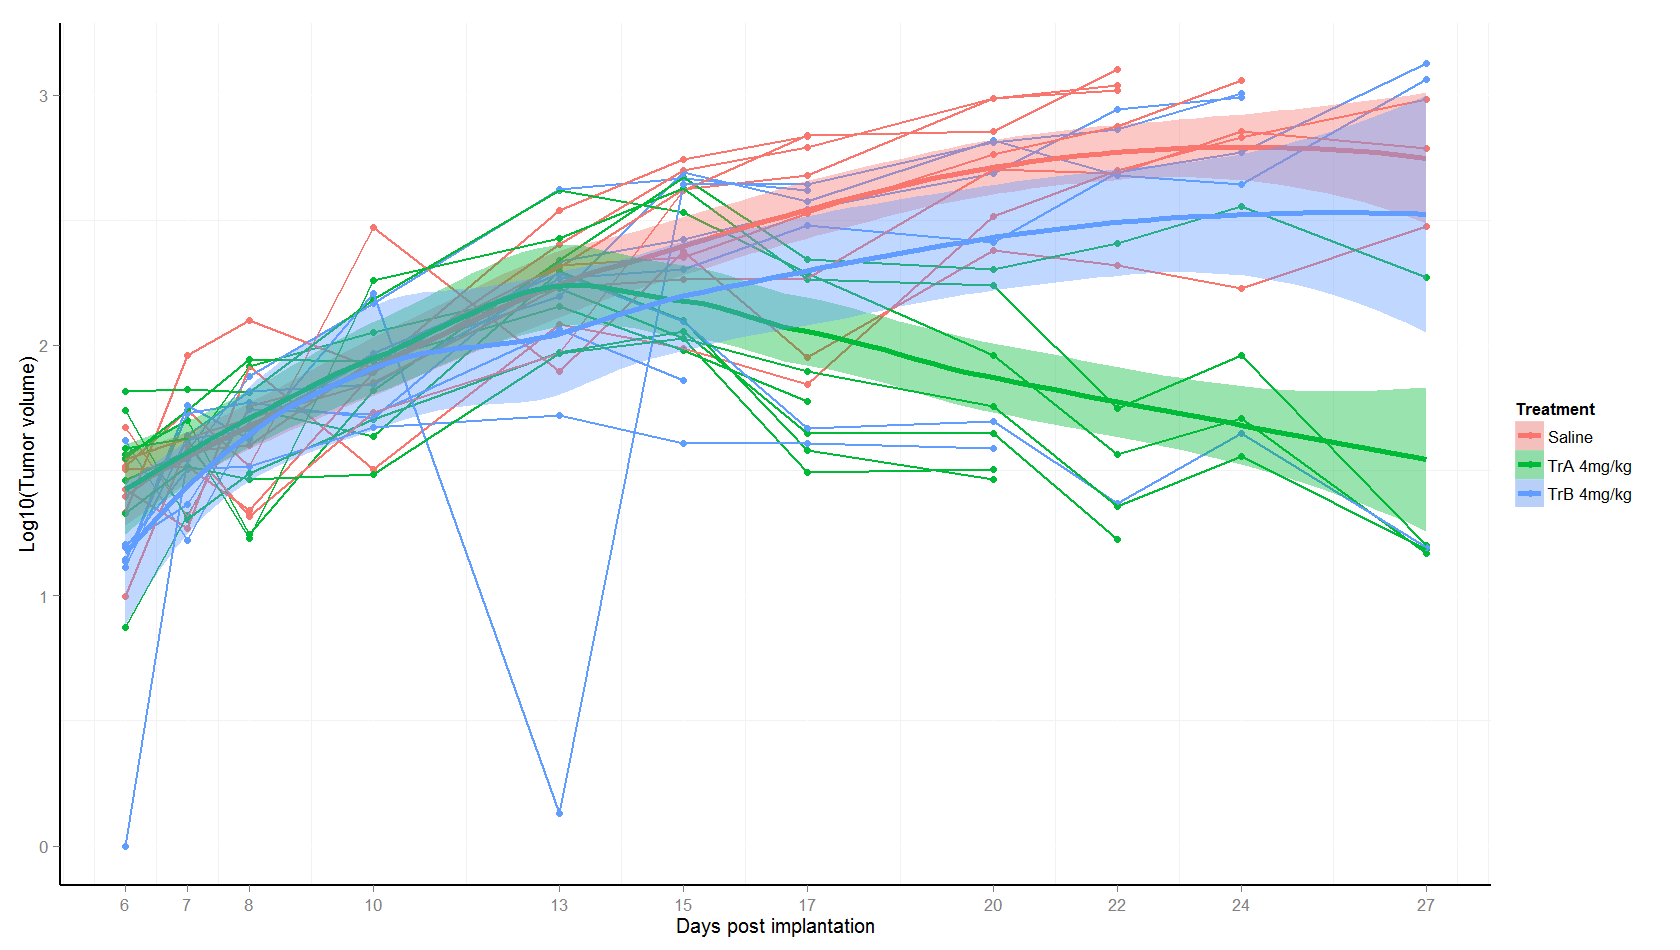
\includegraphics[width=\textwidth]{xenograph/figures/loess_trajectories_log_reduced_follow-up.png}
	\caption{Log$_{10}$-transformed empirical tumour volume (mm$^3$) trajectories with superimposed treatment group LOESS fits with 95\% confidence intervals.
	The smoothing parameter was fixed at 0.75 level.}
	\label{loess_trajectories_log_reduced_follow-up}
\end{figure}


\section{Summary}
\emph{\emph{TBC\ldots}}
